\documentclass[a4paper,11pt,final]{report}

\usepackage[english,francais]{babel}
\usepackage[utf8]{inputenc}
\usepackage[T1]{fontenc}
\usepackage[pdftex]{graphicx}
\usepackage{setspace}
\usepackage{hyperref}
\usepackage[french]{varioref}
\usepackage[final]{pdfpages}
\graphicspath{{images/}}

\newcommand{\reporttitle}{Ordonnancement dans des systèmes distribués}
\newcommand{\reportauthor}{Teddy \textsc{Gilbert} Simon \textsc{Espigolé} Hugo \textsc{Legrand}}
\newcommand{\reportsubject}{Cahier des charges}
\newcommand{\HRule}{\rule{\linewidth}{0.5mm}}
\setlength{\parskip}{1ex}

\hypersetup{
    pdftitle={\reporttitle},
    pdfauthor={\reportauthor},
    pdfsubject={\reportsubject},
    pdfkeywords={rapport} {vos} {mots} {clés}
}

\author{ESPIGOLE Simon & Gilbert Teddy & Hugo Legrand}

\begin{document}

\begin{titlepage}

\begin{center}

\begin{minipage}[t]{0.48\textwidth}
  \begin{flushleft}
    
\includegraphics [width=30mm]{images/logo_eisti.jpg} \\[0.5cm]
    \begin{spacing}{1.5}
      \textsc{\LARGE}
    \end{spacing}
  \end{flushleft}
\end{minipage}
\begin{minipage}[t]{0.48\textwidth}
  \begin{flushright}
  \end{flushright}
\end{minipage} \\[1.5cm]

\textsc{\Large \reportsubject}\\[0.5cm]
\HRule \\[0.4cm]
{\huge \bfseries \reporttitle}\\[0.4cm]
\HRule \\[1.5cm]

\begin{minipage}[t]{0.3\textwidth}
  \begin{flushleft} \large
    \emph{Étudiants :}\\
    \reportauthor
  \end{flushleft}
\end{minipage}
\begin{minipage}[t]{0.6\textwidth}
  \begin{flushright} \large
    \emph{Responsable :} \\
    Juan Angel \textsc{LORENZO DEL CASTILLO} \\
  \end{flushright}
\end{minipage}

\vfill

{\large Pau, le \today}

\end{center}

\end{titlepage}


\tableofcontents

\newpage

\chapter{Introduction}
    \section{Définition du sujet}
    
    L'ordonnanceur (\texttt{scheduler}, en anglais) est l'élément central d'un système d'exploitation multi-processus. L'ordonnancement (\texttt{Scheduling}) définie une méthode par laquelle un travail, \texttt{work}, va être attribué à un processeur pour une partie ou pour la totalité de son fonctionnement. Un ordinateur disposant de ressources limitées et un travail nécessitant des ressources pour fonctionner (puissance de calcul, capacité mémoire, etc...), l'ordonnanceur doit savoir répartir ces travaux afin d'optimiser les ressources matériels à disposition du système. Il peut avoir plusieurs objectifs : 
    
   
    
    \begin{itemize}
        \item Optimisation du nombre de travaux complétés par unité de temps (\texttt{Maximize throughput})
        \item Minimiser le temps de réponse d'un processus en particulier (\texttt{Latency})
        \item Minimiser le temps d'attente des programmes dans la file d'attente (\texttt{Responsiveness})
        \item Égaliser les ressources disponibles pour chaque processus (\texttt{Fairness})
        \item etc...
    \end{itemize}
    
    Il est très difficile d'implémenter un ordonnanceur capable d'optimiser plusieurs aspects à la fois. Par exemple, il faut faire un compromis entre le nombre de travaux complétés et le temps de réponse d'un processus en particulier (\texttt{Throughput} VS \texttt{Latency}). De plus, chaque optimisation de l'ordonnanceur correspond à une stratégie d'ordonnancement spécifique et peut avoir de sérieuses conséquences sur la stabilité et les performances du système d'exploitation.
    
    
    \section{Contexte et objectif}
        
    Dans le cadre du Projet GSI de seconde année d'ingénieur, nous réaliserons un scheduler permettant d'ordonnancer différents processus selon certaines stratégies d’ordonnancement que nous définirons. À réaliser en équipe de 3 personnes, nous utiliserons les méthodes vues en cours pour développer ce projet. Ce projet a pour but de nous faire apprendre la programmation C++ et la programmation parallèle ainsi que distribuée, choses que nous nous efforcerons au mieux de réaliser et de comprendre. De plus, pour la première fois notre outil de gestion de version de code (GitLAB) sera accessible par le responsable du projet, nous devrons donc adapter nos commit à cette situation, les décrire d'une façon plus claire, mais surtout utiliser une convention de nommage comme suit :
    
    \begin{itemize}
        \item Séparer le sujet du corps avec un saut de ligne
        \item Limiter le sujet à 50 caractères
        \item Mettre une majuscule au premier mot du sujet
        \item Ne pas finir le sujet par un point
        \item Utiliser l'impératif pour le sujet
        \item Limiter le corps à 72 caractères par ligne
        \item Utiliser le corps pour expliquer quoi, pourquoi et comment
    \end{itemize}
    
    Nous essaierons donc d'aller au-delà des attentes classiques d'un projet Eistien pour avoir une approche encore plus professionnelle du projet informatique.
    
\chapter{Cahier des charges}

    Les spécifications fournies par le client sont claires : le but de ce projet est d'implémenter un ordonnanceur, un programme permettant d'affecter des tâches à un processeur en fonction de plusieurs options ou paramètres comme : 
    
    \begin{itemize}
        \item Temps d'exécution nécessaire
        \item Puissance de calcul demandé (utilisation du processeur)
        \item Allocation mémoire demandée
    \end{itemize}

    Dans un premier temps  nous nous limiterons à une seule stratégie d'ordonnancement : \texttt{Load balancing} + FIFO. \newline 
    Cette stratégie implémente le principe d'une file d'attente. Le premier processus arrivant sera affecté en premier\footnote{\textsc{FIFO}: \texttt{First In First Out}}. \newline
    Bien que simpliste, cela permettra de garder les ressources occupées et de ne pas surcharger un processeur grâce à la répartition des charges. \newline 
    Néanmoins, nous prévoyons plus tard de permettre à l'utilisateur de choisir sa stratégie d'ordonnancement via une interface terminale simple et intuitive. \newline
    Afin de répartir les charges sur les différents coeurs du processeur, nous utiliserons une option associée au travail que l'on souhaite exécuter. Cela pourrait être, par exemple, une fraction du CPU à utiliser.
    
    Les tâches à effectuer devront être décrites dans un fichier texte. Le fichier pourra avoir la structure suivante : 
    
    \begin{verbatim}
        COMMAND, [OPTIONS]
        --------
        echo "This is a task", 0.1CPU
        ls -l ~/*, 0.2CPU
        rm -rf /, 1CPU
    \end{verbatim}
    
    Ce fichier texte sera analysé et les travaux à effectuer seront placés dans une liste d'attente\footnote{\texttt{Task queue} ou \texttt{pool}, en anglais} dans le programme. Puis, l'ordonnanceur va créer un processus pour chaque commande dans la liste d'attente et les affecter à un \texttt{core} suivant la stratégie d'ordonnancement que l'on aura définie en amont.\newline
    Le programme se termine lorsque la file d'attente ne contient plus aucune tâche à traiter.
    
    La réalisation de ce \texttt{scheduler} se fera sous différentes formes : 
    
    \begin{itemize}
        \item Séquentiel
        \item Parallèle Mono-machine
        \item Parallèle Multi-machine
    \end{itemize}
    
    La première version de l'ordonnanceur sera la plus basique. En effet, les travaux seront assignés les uns après les autres vers le processeur.\newline
    La deuxième implémentation est nettement plus intéressante : le traitement des tâches de la liste se fera en parallèle afin que plusieurs travaux puissent être assigné simultanément. Il faudra donc porter attention aux problèmes de concurrence et de synchronisation qu'il va en résulter. \newline 
    Finalement, il s'agira de répartir les tâches entre différentes machines sur un réseau. Nous détaillerons plus précisément la démarche que nous mettrons en oeuvre dans la partie \texttt{Implémentation} de ce cahier des charges.


\chapter{Implémentation}

    Pour implémenter ce scheduler, nous utiliserons le C++, avec les librairies OpenMP et MPI. Les connections réseau seront faites en IPv6, et le code source sera partagé sur le GitLAB de l'École. Notre groupe utilisera l'environnement de développement CLion (JetBrains) pour toute la rédaction du code source, ainsi que le partage. Pour chaque thread (un par processeur), nous irons chercher une tâche dans le pool de tâches que nous aurons généré au préalable, puis nous la supprimerons. Nous exécuterons la tâche, puis attendrons jusqu'à ce que une nouvelle tâche soit disponible. Le programme s'arrête lorsqu'il n'y a plus de tâche dans le pool de tâches.

\section{Partie séquentielle}

    Pour la partie séquentielle, nous avons pour idée de créer une liste de tâche. Cette liste sera récupérer après un traitement d'analyse de fichier texte afin d'avoir l'ensemble des options d'une tâche. Une fois ceci fait, chaque tâche sera traité l'une après l'autre. Une tâche devra être affectée à un CPU disponible et étant capable d'accueillir la tâche afin de la traiter. Après son affectation, une nouvelle tâche sera récupérée dans la liste. Le programme se terminera quand l'ensemble de la liste sera vide.


\section{Partie parallèle mono-machine}

    Pour la partie parallèle mono-machine, nous allons repartir de la version séquentielle en y ajoutant diverses options. Le traitement des tâches se fera en même temps, une tâche aura un certain poids et se verra affecter un CPU libre et pouvant l'accueillir. Le traitement des tâches se fera de façon parallèle afin de traiter plus rapidement la liste de tâches


\section{Partie parallèle multi-machine}

    La version parallèle de l'ordonnanceur sera réalisée grâce à la librairie MPI en C++. De ce fait, nous serons en mesure d'envoyer un processus directement sur le processeur d'un ordinateur sur le même réseau.
    
    \begin{center}
    \hbox to\hsize{\hss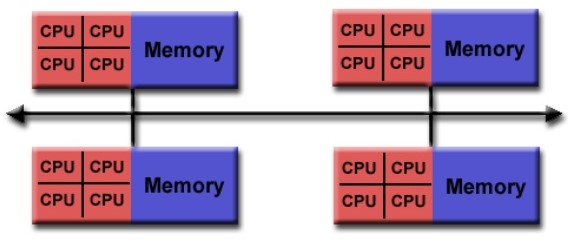
\includegraphics[scale=0.7]{test.jpg}\hss}
    \end{center}

\newpage 

\section{Workflow - Happy path}

    Ci-dessous, vous trouverez le chemin idéal que l'application prendra lors de l'exécution normale du programme : 

    \begin{center}
    \hbox to\hsize{\hss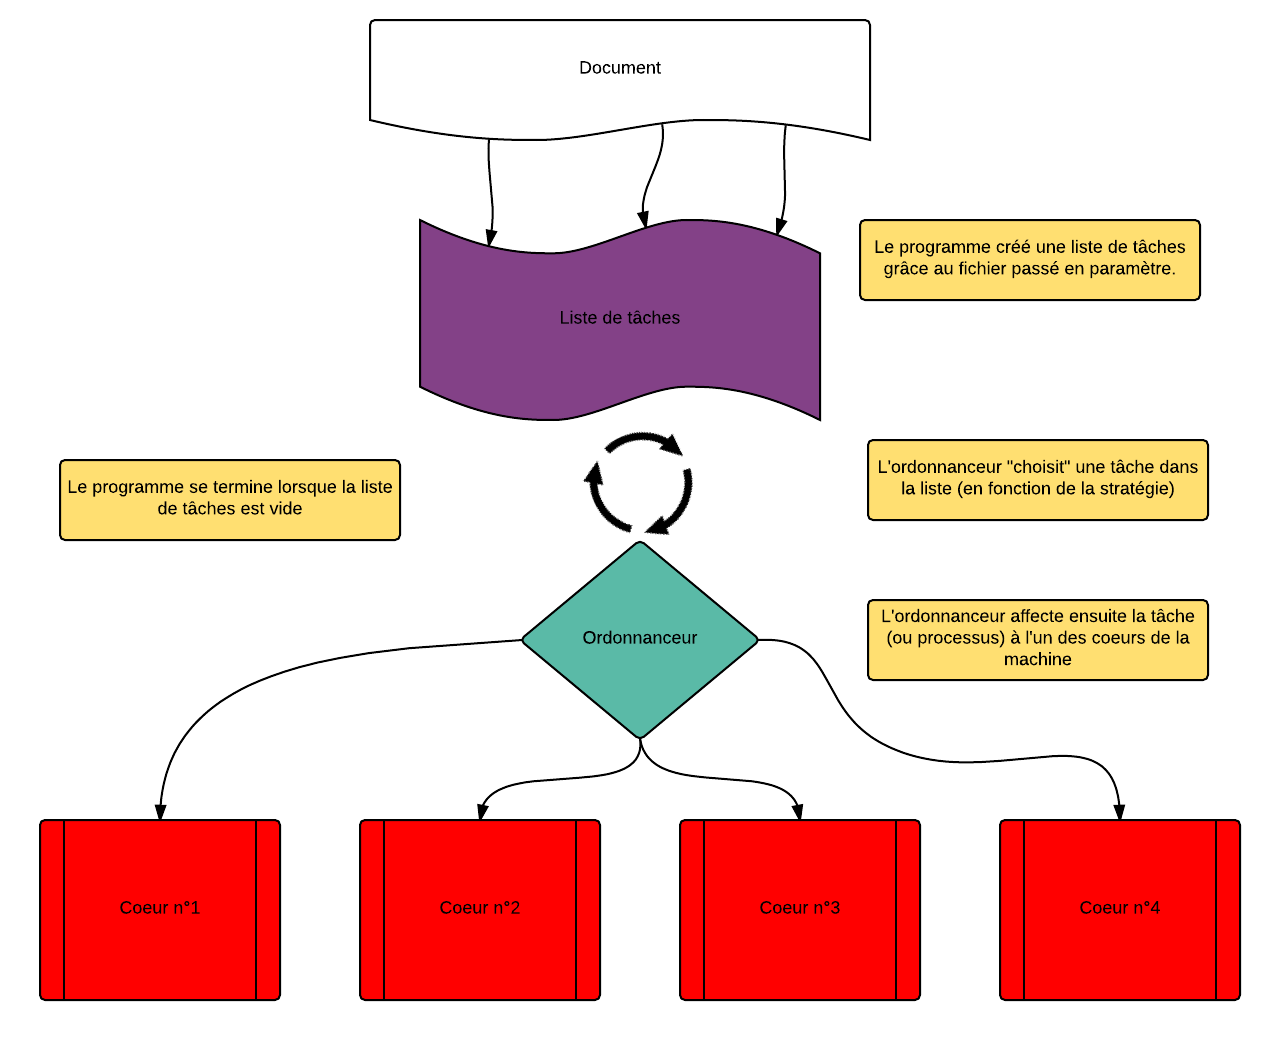
\includegraphics[scale=0.5]{Workflow.png}\hss}
    \end{center}


\chapter{Planning prévisionnel}

    Nous avons prévu un planning pour l'instant simple : nous y avons intégré les grandes étapes du développement sans oublier les phases de test et d'implémentation.

    \begin{center}
    \hbox to\hsize{\hss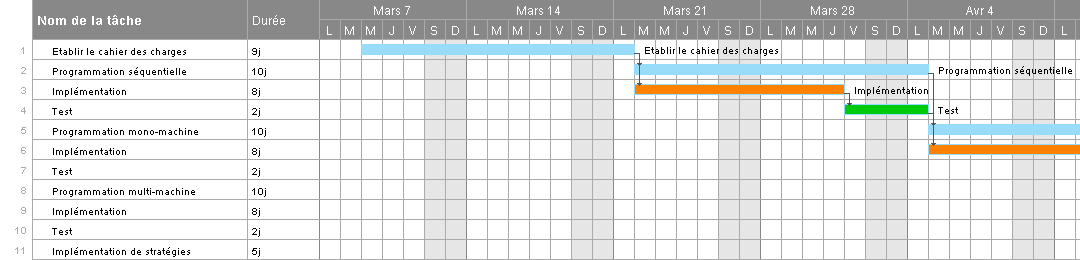
\includegraphics[scale=0.7]{partie1.png}\hss}
    \vspace{2cm}
    \hbox to\hsize{\hss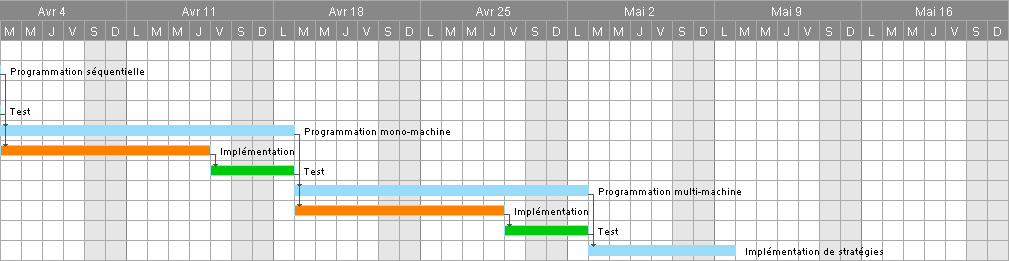
\includegraphics[scale=0.7]{partie2.png}\hss}
    \end{center}

\chapter{Axes d'amélioration}
    
    \section{Amélioration d'interface}

    S'il nous reste du temps après avoir implémenté les principales fonctionnalités, nous choisirons de développer une interface de commande un peu plus développée en premier lieu. Nous souhaitons à terme pouvoir proposer des options nombreuses pour paramétrer au mieux le scheduler.

    \section{Autres stratégies d'ordonnancement}
    
    \subsection{Fixed priority pre-emptive scheduling}
        Une priorité est fixé aux processus. Le scheduler ordonne la file d'attente en fonction de cette priorité. 
        \begin{itemize}
            \item Revient à faire plusieurs FIFO si le range de priorité est limité.
            \item Accorde une réponse quasi immédiate au processus de plus haute priorité
        \end{itemize}
    \subsection{Round-robin scheduling}
        Un jeton\footnote{\texttt{Token}, en anglais} est passé entre les tâches. La tâche qui possède le jeton va s'exécuter pendant un certain temps défini par l'utilisateur, puis l'ordonnanceur va passer le jeton à la tâche suivante. Une fois les processus tous complétés, on arrête.
        
        Cette implémentation risque d'être difficile car il faut sauvegarder le contexte d'un processus avant de le mettre en pause et de passer à un autre processus. Il sera donc intéressant de vérifier les performances de cette stratégies selon les différents temps définis par l'utilisateur.
    
        Nous pourrons par la suite gérer un peu mieux les ressources en instaurant un timeout pour toutes les tâches gérées, qui seront tuées si elles dépassent ce laps de temps. Puis une hiérarchisation des tâches sera effectuée : des priorités seront assignées aux tâches et les plus importantes seront exécutées en premier.

\chapter{Conclusion}

    Ce projet nous servira de base pour apprendre à programmer en C++. Nous nous efforcerons de suivre une méthode rigoureuse tout au long du projet, tant dans la communication inter et intra groupe que dans notre façon de coder.
    De plus, la perspective du développement parallèle et distribué nous intéresse : c'est en effet une nouvelle manière de penser que nous admirons et dont nous avons beaucoup à apprendre. Nous essaierons alors de réaliser au mieux les objectifs que nous nous sommes fixés. \newline
    
    Pour finir, il nous semble important de prendre un peu de recul sur le projet. Bien que nous nous efforcerons d'implémenter la meilleure version de \texttt{scheduler} possible, il semble prétentieux de penser que celui-ci serait viable, au sein d'un système d'exploitation par exemple. En effet, la grande majorité des ordonnanceurs utilisés dans les systèmes informatiques grand public ont des stratégies très différentes de celle que nous programmerons. Bien souvent, leur stratégie consiste en une fusion de plusieurs stratégies connues et optimisées. 

\end{document}